\chapter{Introduction}
\markright{Introduction} % new right header
%======================================================================
\section{Inorganic Chemistry}
%======================================================================

Common distinctions split most chemical compounds into one of two categories: organic and inorganic. Organic molecules typically contain carbon and hydrogen, with or without additional nitrogen, oxygen, phosphorus, sulfur, and the halides. Inorganic chemistry is considered to be the remainder of the molecules possible. While they may include come aspect of organic chemistry (especially in organometallic molecules), the main structural motif or reactive center is a non-organic feature. These inorganic compounds can range from compounds such as lithium or grignard reagents with significant organic influence, to metallic alloys or mineral compounds. With such a wide range of possibilities, inorganic chemistry has many facets. A widely active research area is the development and testing of transition metal complexes for catalytic, photophysical, biochemical or manufacturing uses.
%======================================================================
\section{Photochemistry \& Catalysis}
%======================================================================

Transition metal complexes were first identified to be catalytically active in \_, when \_ first demonstrated the use of \_ with a \_ ligand for the \_ of \_ \/autocite\{ref\}. This and similar types of complexes have grown into multi-billion dollar industries, responsible for the production of megatons of plastics in the last \_ years. Similar complexes have been used for \_ and \_ purposes.

Many of these catalysts are active for photocatalysis. In typical transition metal complexes, the interaction between the metal atom(s) and the ligands cause significant electron mobility upon the absorbtion of incident photons. 
%======================================================================
\section{Rhenium}
%======================================================================

Rhenium compounds display a broad scope of applications ranging from catalysis\autocite{dudle2011, jain2008, kuninobu2011} to radiopharmaceutical applications\autocite{bartholoma2009, schibli2002}, as well as possessing interesting fundamental photophysical properties\autocite{coogan2009}. Since the mid-1970's, complexes containing the $\alpha$-diimine Re\textsuperscript{I} tricarbonyl core have attracted a great deal of attention due to their attractive photochemical properties with pseudo-octahedral \textit{fac}-[L\textsubscript{2}Re(CO)\textsubscript{3}X] and \textit{fac}-[L\textsubscript{2}(L')Re(CO)\textsubscript{3}]\textsuperscript{+} complexes being the dominant species\autocite{giordano1979, sacksteder1990, caspar1983, yam2001, feliz1998, ruiz1996, lin1992, hino1992, walters2002, striplin2001}. A large family of compounds with these formulations have been accessed by the addition of chelating diimine $\sigma$-donor ligands to [Re(CO)\textsubscript{5}X] with the quantitative replacement of two \textit{cis} carbonyls in the Re\textsuperscript{I} starting material\autocite{giordano1979, martin2011, abel1959, kirkham1965, zingales1967, gamelin1994, marti2005, morse1976, giordano1978}. Significantly, these reactions form only bidentate coordinated ligands with \textit{facial} tricarbonyl isomers as products even when a potentially tridentate $\sigma$-donor, such as bis(imino)pyridine or 2,2':6',2''-terpyridine are employed in the reaction (Figure \ref{fig.terdentateligands})\autocite{granifo1999, orrell1997, abel1993}. These robust species have been examined for potential applications in organic light-emitting diodes (OLEDs)\autocite{gong1998}, chemosensors and biotechnology probes\autocite{lo2010, lin2007, slone1995, beer1999, beer2003}, fluorescence microscopy imaging of cells\autocite{lo2010, amoroso2008, amoroso2007}, and the photochemical reduction of CO\textsubscript{2} to CO\autocite{hawecker1983, hawecker1986, takeda2010, christensen1992, sullivan1985}. Among the key photophysical features of these $\alpha$-diimine Re\textsuperscript{I} compounds is the electron transfer capability of this system and the interplay between the Re center and the well-known non-innocent redox-activity of the ligands\autocite{caulton2012}.

\begin{figure}[!htbp]
 \begin{center}
  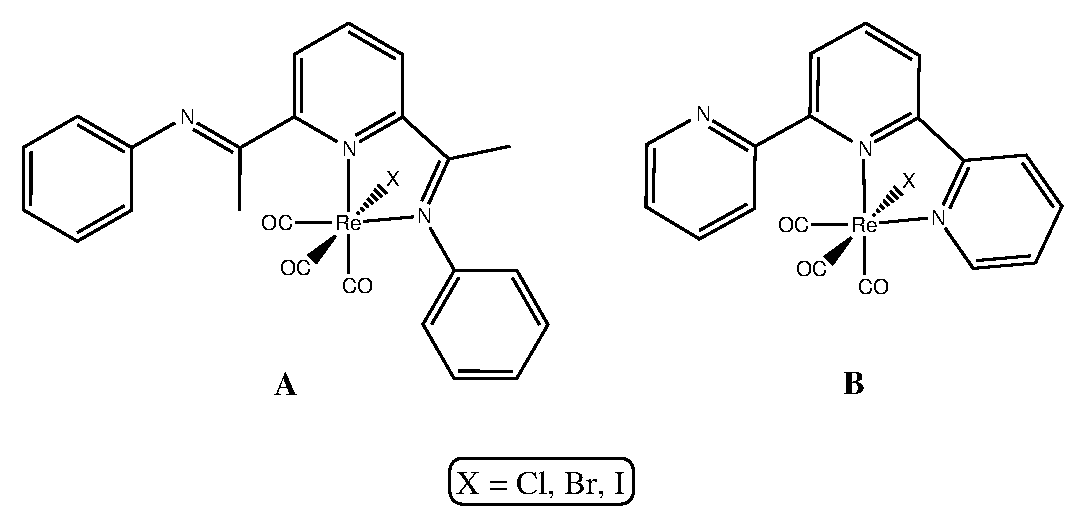
\includegraphics[clip=true, width=110mm]{images/terdentateligands.eps}
 \end{center}
\caption[Two common bidentate complexes using terdentate ligands]{Two common \textit{fac}-[L\textsubscript{2}Re(CO)\textsubscript{3}X] complexes with terdentate $\sigma$-donor ligands: L = bis(imino)pyridine (\textbf{A}) and 2,2':6',2''-terpyridine (\textbf{B})}
\label{fig.terdentateligands}
\end{figure}

Further development of this chemistry has been restricted by the limited structural and electronic variability of the common pseudo-octahedral \textit{fac}-[L\textsubscript{2}ReX(CO)\textsubscript{3}] (L\textsubscript{2} = $/alpha$-diimine) products. While these systems continue to receive considerable attention, studies detailing the coordination chemistry of the meridionally-coordinated tridentate triimine Re\textsuperscript{I} dicarbonyl core are quite limited\autocite{jurca2013}. For example, while $\kappa$\textsubscript{3}-(terpy)Re(CO)\textsubscript{2}Cl was initially reported in 1988\autocite{juris1988}, closer analysis of the reported analytical data (including \textsuperscript{1}H NMR) indicate that this compound is more likely $\kappa$\textsubscript{2}-LRe(CO)\textsubscript{3}Cl. A more recent report for this compound provides spectroscopic details of this species as well as the preliminary report for the generation of [($\kappa$\textsubscript{3}-(terpy)Re(CO)\textsubscript{2}L’]\textsuperscript{+} cations (L = PPh\textsubscript{3}, PEt\textsubscript{3}, NC\textsubscript{5}H\textsubscript{5}, and NCCH\textsubscript{3})\autocite{black2012}. Finally, the \textsuperscript{1}H NMR data for ($\kappa$\textsubscript{3}-(terpy)Re(CO)\textsubscript{2}Br) has been reported\autocite{abel1993}.

In order to fully exploit the potential of this versatile family of compounds, the limits imposed by the bidentate coordination need to be addressed. Furthermore, it would appear that, on the basis of the tridentate ligands that have been investigated, the concerted effort to produce the tridentate species has been unsuccessful. Attracted by this challenge we sought to synthesize, crystallographically authenticate, and investigate the photophysical properties of low-valent rhenium pincer complexes displaying an N,N',N''-chelated terpyridine array. 

We recently reported the conversion of bidentate bis(imino)pyridine complexes 2,6-\{2,6-Me\textsubscript{2}C\textsubscript{6}H\textsubscript{3}N=CPh\}\textsubscript{2}(NC\textsubscript{5}H\textsubscript{3})Re(CO)\textsubscript{3}X  (X = Cl, Br) into tridentate pincer ligand compounds, 2,6-\{2,6-Me\textsubscript{2}C\textsubscript{6}H\textsubscript{3}N=CPh\}\textsubscript{2}(NC\textsubscript{5}H\textsubscript{3})Re(CO)\textsubscript{2}X (X = Cl, Br)\autocite{jurca2013}. This transformation was performed in the solid-state by controlled heating of these bidentate species above 200$^\circ$C in a tube furnace under a flow of nitrogen gas giving excellent yields ($\geq$~95\%). These compounds defined a new coordination environment for Re\textsuperscript{I} carbonyl chemistry where the metal center is supported by a planar, tridentate pincer coordinated bis(imino)pyridine ligand. 

Complexes of 2,2':6',2''-terpyridine (terpy) are of interest due to the conceptual relationship to established bis(imino)pyridine compounds\autocite{russell2010, tondreau2012}. Herein, we provide rational synthetic procedures to these novel species as well as their characterization and analysis of their visible electronic transitions. These results will broaden the accessibility of such compounds for investigation and application. This report for the unconventional but accessible synthesis of tridentate pincer complexes promises to enhance the versatile chemistry of Re\textsuperscript{I} and yield new venues for exploration.
